\subsection{GMM (Gaussian Mixture Model)}
GMM, или модель гауссовых смесей, наследует идеи байесовских сетей в том смысле, что она может быть легко представлена в рамках парадигмы графического моделирования.

Пример графической модели, представляющей гауссову смесь, показана на рисунке~\ref{fig:spec:GmmRepresentation}. Здесь $q_k\in \{1,\dots,M\}$, $\theta = (\pi_1,\dots,\pi_M,\mu_1,\dots,\mu_M,\Sigma_1,\dots,\Sigma_M)$. Закрашенные узлы представляют наблюдаемые непрерывные переменные, $y_k$ для момента времени $k$. Незакрашенные узлы, $q_k$, представляют $M$ ненаблюдаемых дискретных переменных, условная вероятность которых может быть вычислена на основе наблюдаемых данных. Параметры, содержащие $\theta$, могут быть выражены как функция от этих условных вероятностей и от других похоже сформированных оценок для каждой из $M$ гауссовых смесей, включая весовые коэффициенты смесей ($pi_i$), математические ожидания ($mu_i$) и матрицы ковариации ($\Sigma_i$).

\begin{figure}[h]
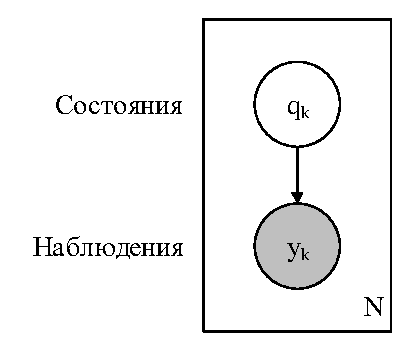
\includegraphics{gmm}
\caption{Графическое представление GMM без учителя}
\label{fig:spec:GmmRepresentation}
\end{figure}

Для использования данного метода требуется выполнение двух гипотез, представленных ниже.

\uline{Гипотеза о природе данных}: тестовые примеры появляются случайно и независимо, согласно вероятностному распределению, равному смеси распределений кластеров. Данное условие отображено в формуле~\eqref{eq:spec:GMM:Condition1}.

\begin{equation} \label{eq:spec:GMM:Condition1}
p(x) = \sum_{c\in C}^{} w_c p_c(x), \sum_{c\in C}^{} w_c = 1\text{,}
\end{equation}
\begin{description}
	\item[где $w_c$]~---~вероятность появления объектов из кластера $c$;
	\item[$p_c$]~---~плотность распределения кластера $c$.
\end{description}

\uline{Гипотеза о форме кластеров}: каждый кластер $c$ описывается $d$-мерной гауссовской плотностью с центром $\mu_c = \{\mu_{c1},\dots,\mu_{cd}\}$ и диагональной матрицей ковариации $\Sigma_c = diag(\sigma^2_{c1},\dots,\sigma^2_{cd})$ (т.е. по каждой координате своя дисперсия).

В этих предположениях для определения аномалий получается задача разделения смеси гауссовых распределений. Для этого обычно используется EM-алгоритм (expectation-maximization)~\cite{MartinCompUnsupervisedDetectionMethods}. Подробное описание данного алгоритма представлено в~\cite{KorolevEMAlgo}.

EM-алгоритм используется в математической статистике для нахождения оценок максимального правдоподобия параметров вероятностных моделей, в случае, когда модель зависит от некоторых скрытых переменных. Каждая итерация алгоритма состоит из двух шагов. На \textit{E-шаге (expectation)} вычисляется ожидаемое значение функции правдоподобия, при этом скрытые переменные рассматриваются как наблюдаемые. На \textit{M-шаге (maximization)} вычисляется оценка максимального правдоподобия, таким образом увеличивается ожидаемое правдоподобие, вычисляемое на E-шаге. Затем это значение используется для E-шага на следующей итерации. Алгоритм выполняется до сходимости.

Формальная постановка задачи разделения смеси гауссовых распределений выглядит следующим образом. Задана выбора $X^l$ случайных и независимых наблюдений из смеси $p(x)$, в которой описание $i$-го элемента есть вектор $x_i\in \mathbb{R}^n$. Принята модель, в которой каждая компонента смеси есть гауссиана с параметрами $\mu$ и $\Sigma$, и известно число компонентов смеси~---~$K$. Смесь показана в формуле~\eqref{eq:spec:GMM:Mixture}.

\begin{equation} \label{eq:spec:GMM:Mixture}
p(x) = \sum_{n=1}^{K} \pi_k N(x|\mu_k,\Sigma_k).
\end{equation}

Требуется оценить вектор параметров $\theta = (\pi_1,\dots,\pi_M,\mu_1,\dots,\mu_M,\Sigma_1,\dots,\Sigma_M)$, доставляющий максимум функции правдоподобия~\eqref{eq:spec:GMM:LikelihoodFunc}.

\begin{equation} \label{eq:spec:GMM:LikelihoodFunc}
\ln p(X|\pi,\mu,\Sigma) = \sum_{n=1}^{N} \ln \left\{\sum_{k=1}^{K} \pi_k N(x_n|\mu_k,\Sigma_k)\right\}
\end{equation}

Оптимальные параметры отыскиваются последовательно с помощью итерационного EM-алгоритма. Основная идея~–--~вводится вспомогательный вектор скрытых переменных. Это позволяет свести сложную оптимизационную задачу к последовательности итераций по пересчету коэффициентов (скрытых переменных по текущему приближению вектора параметров~---~E-шаг) и максимизации правдоподобия (с целью найти следующее приближение вектора~---~М-шаг).

В начале работы алгоритма задаются параметры начального приближения $\theta_0$. Далее итеративно выполняется следующая пара процедур:

\uline{E-шаг}: используя текущее значение вектора параметров $\theta$, вычисляется значение вектора скрытых переменных $\gamma$ по формуле~\eqref{eq:spec:GMM:HiddenVars}.

\begin{equation} \label{eq:spec:GMM:HiddenVars}
\gamma_{nk} = \frac{\pi_k N(x_n|\mu_k,\Sigma_k)}{\sum_{j=1}^{K} \pi_j N(x_n|\mu_j,\Sigma_j)}
\end{equation}

\uline{M-шаг}: переоценка вектора параметров по формулам~\eqref{eq:spec:GMM:newParams}, используя текущее значение вектора скрытых переменных.

\begin{subequations} \label{eq:spec:GMM:newParams}
\begin{equation} %\label{eq:spec:GMM:newMu}
\mu_k^{new} = \frac{1}{N_k} \sum_{n=1}^{N} \gamma_{nk} x_n \text{,}
\end{equation}
\begin{equation} %\label{eq:spec:GMM:newSigma}
\Sigma_k^{new} = \frac{1}{N_k} \sum_{n=1}^{N} \gamma_{nk} (x_n - \mu_k^{new})(x_n-\mu_k^{new})^T \text{,}
\end{equation}
\begin{equation} %\label{eq:spec:GMM:newPi}
\pi_k^{new} = \frac{N_k}{N} \text{,}
\end{equation}
\begin{equation} %\label{eq:spec:GMM:newN}
N_k = \sum_{n=1}^{N} \gamma_{nk} \text{,}
\end{equation}
\end{subequations}

Процедура останавливается после того, как норма разности векторов скрытых переменных на каждой итерации не будет превышать заданную константу~$\Delta$. Условие останова показно в~\eqref{eq:spec:GMM:StopCondition}.

\begin{equation} \label{eq:spec:GMM:StopCondition}
\delta_{max} = \max \left\{\delta_{max},|\gamma_{nk} - \gamma_{nk}^0|\right\} \leq\Delta
\end{equation}

Блок-схема алгоритма приведена в приложении~\ref{app:GMM:EMScheme}.

Для поиска аномалий могут быть использованы различные варианты моделей гауссовых смесей, например, модели для одного датчика системы (одномерный случай), либо для нескольких датчиков с учётом корреляции между ними (многомерный случай).

Оценка метода в применении к контролю и диагностике КА дана в~\cite{MartinCompUnsupervisedDetectionMethods}~и~\cite{MartinUnsupervisedAnomDetectForLiquid}.

Преимущества метода:
\begin{itemize}
	\item возможность построения независимой модели для каждого датчика, что обеспечивает более точную диагностику;
	\item модель можно представить в графической форме.
\end{itemize}

Недостатки:
\begin{itemize}
	\item строгие требования к исходным данным: если выборка не подчиняется нормальному распределению, то использование данного метода невозможно;
	\item метод не работает с выборками, имеющими коррелированные параметры;
	\item необходимость вручную задавать число кластеров, которое весьма трудно поддаётся определению в многомерных случаях и при больших объёмах данных~\cite{MartinUnsupervisedAnomDetectForLiquid}.
\end{itemize}